%&pdflatex
%% filename: amsart-template.tex, version: 2.1
\documentclass{amsart}
\usepackage{amscd}
\usepackage{amsmath}
\usepackage{amssymb}
\usepackage{amsthm}
\usepackage{bbm}
\usepackage{bbold}
\usepackage{bm}
\usepackage{fontenc}
\usepackage{graphicx}
\usepackage{hyperref}
\usepackage{inputenc}
\usepackage{mathrsfs}
\usepackage{mathtools}

\hypersetup{linkcolor=blue,citecolor=red,filecolor=dullmagenta,urlcolor=blue}

\newtheorem{conj}{Conjecture}
\newtheorem{corollary}[theorem]{Corollary}
\newtheorem{definition}[theorem]{Definition}
\newtheorem{definition}{Definition}
\newtheorem{example}[theorem]{Example}
\newtheorem{lemma}[theorem]{Lemma}
\newtheorem{notation}{Notation}
\newtheorem{proposition}[theorem]{Proposition}
\newtheorem{remark}[theorem]{Remark}
\newtheorem{remark}{Remark}
\newtheorem{theorem}{Theorem}[section]
\newtheorem{xca}[theorem]{Exercise}
\numberwithin{equation}{section}
\setlength{\parindent}{0pt} % turn off auto-indent
\theoremstyle{definition}
\theoremstyle{remark}

\DeclarePairedDelimiter\abs{\lvert}{\rvert}%
\DeclarePairedDelimiter\norm{\lVert}{\rVert}%
\newcommand{\bnxk}{{\mathrm{N}}(x,k)}
\newcommand{\pd}{\frac{\partial}{\partial}}
\newcommand{\px}[1]{\pi(x,{#1})}
\newcommand{\Px}[1]{\Pi(x,{#1})}
\newcommand{\snxk}{\pi(x,k)}

\graphicspath{ {./} }

\begin{document}

\title{Assignment 3: Neural Turing Machines [IFT6135]}

\author{Joseph D. Viviano, Marzi Mehdizad, Johnathan Guymont}
\address{Universit\'e de Montr\'eal}
\curraddr{}
\email{joseph@viviano.ca, jonathan@guymont.com, marzieh.mehdizadeh@gmail.com}
\thanks{}
\date{March 2018}

\maketitle

\section{Filling the Gaps} \\

\textbf{Writing Parameters}\\
In the writing head we have two parameters ($\bm{e_t}$ and $\bm{a_t}$). Writing involves two steps : erasing and adding\\
\textbf{Erasing:} In order to erase the old data a writing head needs  the erase vector $\bm{e_t}$ of size $M$ whose elements are values between $0$ and $1$, in addition to our length-$N$ normalized weight vector $w_t$. The erase vector is used in conjunction with the weight vector to specify which elements in a row should be erased, left unchanged, or something in between. If the weight vector tells us to focus on a row, and the erase vector tells us to erase an element, the element in that row will be erased.
$$\tilde{M_t}(i)\leftarrow M_{t-1}\left[\bm{1}-w_t(i)\bm{e_t}\right]$$
\textbf{Remark:} In order to update the value of $\bm_{e_t}$ we need to use the Sigmoid function after each back propagation to keep the elements of $\bm{e_t}$ between $0$ and $1$.\\
\textbf{Adding:} After $M_{t−1}$ has been converted to $\tilde{M}$, the write head uses a length-{M} add vector $\bm{a_t}$ to complete the writing step.
$$M_t(i)\leftarrow \tilde{M_t}+w_t(i)\bm{a_t}.$$



\textbf{Addressing Parameters}\\
We have a $4$ stage-process and $5$  parameters ($\bm{k_t},\bm{\beta_t}, \bm{g_t}, \bm{s_t}, \bm{\gamma_t}$) to get the controller output. \\
\textbf{Stage 1 (Content addressing parameters ):} The first stage is to generate a weight vector, based on how similar each row of memory is to a vector $\bm{k_t}$ emitted by controller. We introduce a the vector $W_t^c$ as the \textit{content vector}. The content vector allows the controller to choose values which are similar to previous values, which is called content based addressing.\\
For each head , the controller produces a \textit{key vector} $\bm{k_t}$ that will be compared to each row of $M_t$ by using a measure. this measure can be the euclidean measure , but here the authors used the cosine measure defined as follows
$$K(u,v):= \frac{u.v}{||u||.||v||}$$
The $i$th row of the content weight vector is obtained by the following formula

$$w_t^c(i)\leftarrow \frac{\exp\left(\bm{\beta_t} K(\bm{k_t},M_t(i)\right)}{\sum_j \exp \left( \bm{\beta_t}K(\bm{k_t},M_t(j))\right)}. $$
The parameter $\bm{\beta_t}$ which is called \textit{key strength}, is a scalar constrained in the  $(0,\infty)$. It is used to show that how focused the content weight should be. We have two cases for the values of $\bm{\beta_t}$:\\
$\textbf{i:}$ If $\bm{\beta_t }\leq1$: In this case the values of weight vector spread over a large area. \\
$\textbf{ii:}$If $\bm{\beta_t} >1$: In this case, As the values of $\bm\beta_t$ get larger and larger then the weight vector will be concentrated on the most similar row in memory.\\
\textbf{Example:}
let $\bm k_t= (3\quad 2 \quad1)$ and the memory matrix is as follows:
\[M_t=
\begin{bmatrix}
    1     & 2& 3 & 1 &0&1 \\
    1      & 1 & 2 & 4 & 0&0 \\

    2  & 4& 1& 5 & 1&0
\end{bmatrix}
\]
If $\bm {\beta_t} \rightarrow 0$ then
$$w_t^c \rightarrow (0.16\quad  0.16\quad 0.16\quad .16\quad 0.16\quad 0.16).$$
Let $\bm{\beta_t}=5$, then
$$w_t^c= (0.16\quad 0.1\quad 0.47\quad 0.08 \quad0.13\quad 0.17).$$
Let $\bm{\beta_t}=50$
$$w_t^c= (0\quad 0\quad 0\quad 1\quad 0\quad 0)$$
\textbf{Remark:} To update the value of $\bm{\beta_t}$ in each back propagation of our model we use the \textit{Softplus} funtion over the value $\bm{\beta_t}$ obtained by back propagation process to have get a non-negative value. So the updated beta will be:

$$\bm{\beta_t'}= log (1+e^{\bm{\beta_t}})$$\\
\textbf{Stage 2 (interpolation parameter):} Sometimes the our variables are stored in different addresses and we don't care about their values , because the controller will retrieve them from and perform the desired algorithm. So the variables are addressed by location and not the content. So in this stage we decide when we should use or ignore the content-based addressing . We introduce the scalar $\bm{g_t}\in(0,1)$ named \textit{interpolation gate} that combine $w_t^c$ with the previous step weight vector $w_{t-1}$ and produce the gated weighting  $w_t^g$ defined as follows
$$w_t^g \leftarrow \bm{g_t}w_t^c +(1-\bm{g_t})w_{t-1}$$
So as we observe in this formula:\\
$\textbf{i:}$ If $\bm{g_t}\rightarrow 0$ then the weight in previous stage is chosen and $w_t^c$ is completely ignored.\\
$\textbf{ii:}$ if $\bm{g_t}\rightarrow 1$ then the content base addressing is selected and the previous step's weight will be ignored.\\
\textbf{Example:} Let $w_t^c= (0 \quad 0 \quad 1\quad  0\quad 0 \quad 0)$ and $w_{t-1}= (0.9 \quad 0.1 \quad 0 \quad 0\quad 0\quad 0)$\\
If $g_t\to 1$ then
$$w_t^g \to (0\quad 0\quad 1\quad 0\quad 0\quad 0)$$
If $g_t= 0.5$ then
$$w_t^g= (0.45 \quad 0.05 \quad 0.5 \quad 0\quad 0)$$
If $g_t \to 0$ then
$$w_t \to (0.9 \quad 0.1 \quad 0\quad 0\quad 0\quad 0).$$
\textbf{Remark:} To update the value of $\bm{g_t}$ in each back propagation of our model we use the \textit{Sigmoid} function over the value $\bm{g_t}$ obtained by back propagation process to have get a  value between $0$ and $1$. So the updated $\bm{g_t}$ will be:
$$\bm{g_t'}=sigmoid(\bm{g_t})$$

\textbf{Stage 3(Convolutional shift parameter):} After interpolation stage, each head emits a shift weighting $\bm{s_t}$. This parameter makes the controller able to shift concentrating to other rows. The range of shift is given as a parameter. For example if it is between $-1$ and $1$, then the shift range size is $3$ (shift forward a row(+1), stay in the same row (0), shift backward a row(-1)).\\
We perform a shift modulo $N$ such that a shift forward for the last row of the memory shift the head's attention to the the first rows. \\
the following convolutional shift is performed to produce the shifted weight ${\tilde{w}_t}$

$$\tilde{w}_t(i)\leftarrow \sum_{j=1}^{N-1} w_t^g(j)\bm{s_t}(i-j)$$

\textbf{Example:} let $\bm{s_t}$ have three elements corresponding to the degree to which shifts of -1, 0 and 1 are performed, assume that we are working on the element with  index $3$,  and $w_t^g$ has $5$ entries. So we have

%$$\tilde{w_t}(3)=w_t^g (0) s_t((3-0)%5)+ w_t^g(1) (s_t(3-1)%5)+ w_t^g(2) s_t((3-2)%5)+  w_t^g(3) s_t((3-3)%5)$$

let $w_t^g= (0.45 \quad 0.05 \quad 0.5 \quad 0 \quad 0)$

If $s_t= (1 \quad 0\quad 0)$ (we note that $\sum_i s_t(i)=1$) then we have
$$\tilde{w_t}= ( 0.05 \quad 0.5 \quad 0\quad 0 \quad 0.45)$$ which means that all element shifted to the left.

If $s_t= (0 \quad 0\quad 1)$ (we note that $\sum_i s_t(i)=1$) then we have
$$\tilde{w_t}=  (0\quad 0.45 \quad 0.05 \quad 0.5 \quad 0)$$ which means that all element shifted to right.
If $s=(0.5\quad0\quad  0.5)$
Then $$\tilde{w_t}= (0.25\quad 0.425 \quad 0.025\quad  0.25 \quad 0 \quad 0.225)$$
which means that each number gives half of its value to the right and the other half to the left.

\textbf{Stage 4(sharpening):} The fourth stage, sharpening is used to prevent the shifted weight $\tilde{w}_t$ from blurring, so we use a scalar $\bm{\gamma_t}>1$ to sharpen the weight obtained from the previous stage.

$$w_t(i) \leftarrow \frac{\left(\tilde{w}_t(i)\right)^{\gamma_t}}{\sum_j \left(\tilde{w_t}(j)\right)^{\gamma_t}}$$

\textbf{Example:}\\
let $\tilde w_t = (0\quad 0.45 \quad 0.05 \quad 0.5 \quad 0\quad 0)$
If $\gamma_t= 0$ then
$$w_t= (0.16 \quad 0.16 \quad 0.16\quad 0.16 \quad 0.16 \quad 0.16)$$
In this case (when the value of $\gamma_t <1$), Then $w_t$ will be more blurred.
If $\gamma_t =5$ then

$$w_t= (0 \quad 0.37 \quad 0 \quad 0.62 \quad 0 \quad 0).$$
In this case the values are more sharpened but not enough.

If $\gamma_t=50$ then
$$w_t= (0\quad 0\quad 0\quad 1\quad 0\quad 0)$$
In this case since the value of $\gamma_t$ is large enough then the array will be completely sharpened.

\textbf{Remark:} To update the value of $\bm{\gamma_t}$ in each back propagation of our model we use the \textit{Softplus} function over the value $\bm{\gamma_t}$ obtained by back propagation process to have get a value non-negative. So the updated $\bm{\gamma_t}$ will be:
$$\bm{\gamma_t'}=1+Softplus(\bm{\gamma_t})$$
We add $1$ to the Softplus function to have the updated value bigger than $1$, in order of sharpening and not blurring. \\


\begin{figure}[h]
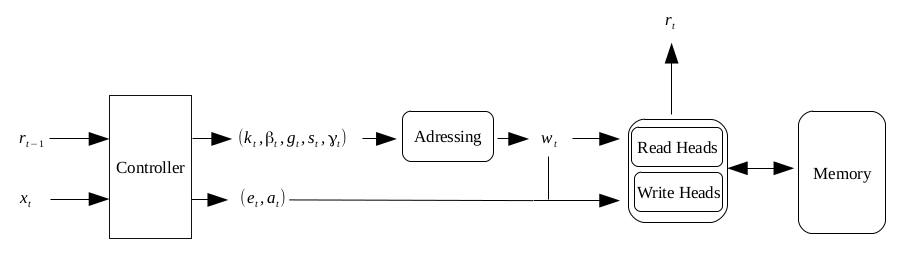
\includegraphics[width=100mm]{ntm_graph}
\caption{Ineraction between the controller and read/write heads.}
\label{Figure 1}
\end{figure}

}}
\section{Implementing the Neural Turing Machine}

Our implementation was forked from \url{https://github.com/loudinthecloud/pytorch-ntm}.
The code can be found at \url{https://github.com/josephdviviano/pytorch-ntm}.\\

\subsection{Parameters} \\

As requested, all models made use of a single 100-node layer (for the NTM models,
this layer was in the controller, for the LSTM, this layer was the hidden layer).
Both NTM models used a single read and write head. \\

\begin{enumerate}
  \item{LSTM-NTM: number of parameters = 62860}
  \item{MLP-NTM: number of parameters = 13260}
  \item{LSTM (baseline): number of parameters = 45408}
\end{enumerate} \\

\subsection{Hyperparameters Chosen} \\

The same hyperparameters were used for all models to facilitate comparison. All
models were trained on 40000 sequences, with a random length between 1 and 20.
We used the rmsprop optimizer, with a learning rate of 0.0004, momentum of 0.9,
and alpha of 0.95. The loss was binary cross entropy. \\

Please see figures 2-4 for the convergence of the three models (LSTM-NTM,
MLP-NTM, and LSTM baseline) using these hyperparameters, respectively. \\

\begin{figure}[h]
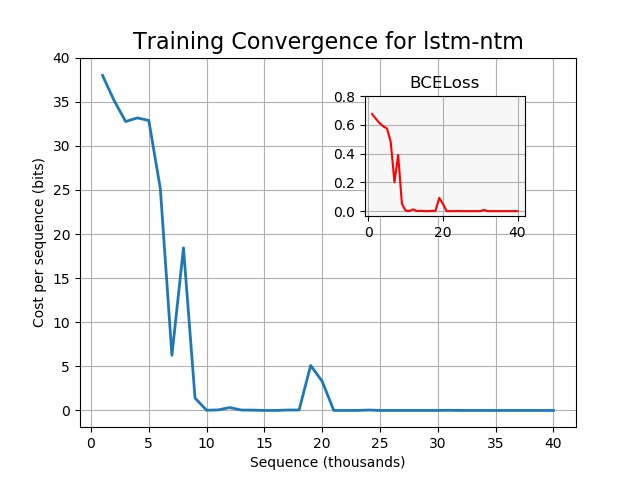
\includegraphics[width=100mm]{outputs/lstm-ntm_convergence}
\caption{Training curve of LSTM-NTM.}
\label{Figure 2}
\end{figure}

\begin{figure}[h]
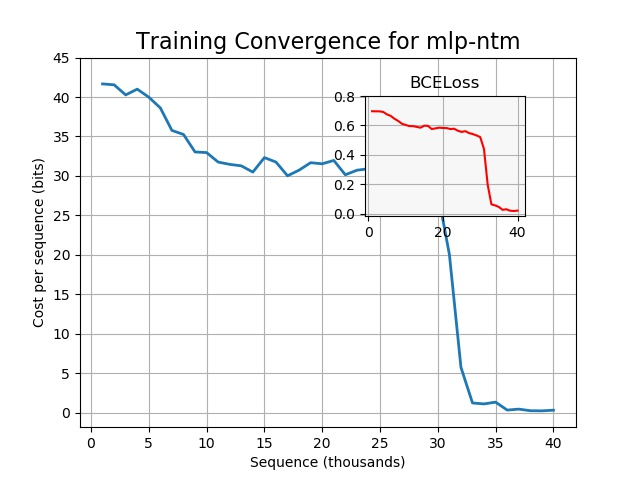
\includegraphics[width=100mm]{outputs/mlp-ntm_convergence}
\caption{Training curve of MLP-NTM.}
\label{Figure 3}
\end{figure}

\begin{figure}[h]
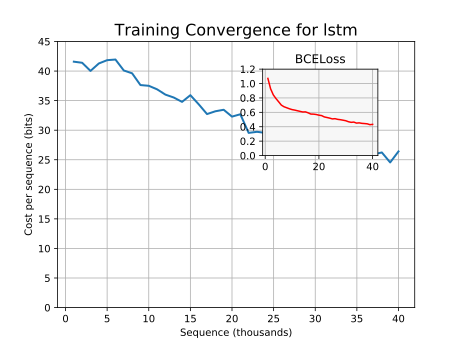
\includegraphics[width=100mm]{outputs/lstm_convergence}
\caption{Training curve of LSTM baseline.}
\label{Figure 4}
\end{figure}

Furthermore, the curve per sequence size can be seen for each in figures 5-7:\\

\begin{figure}[h]
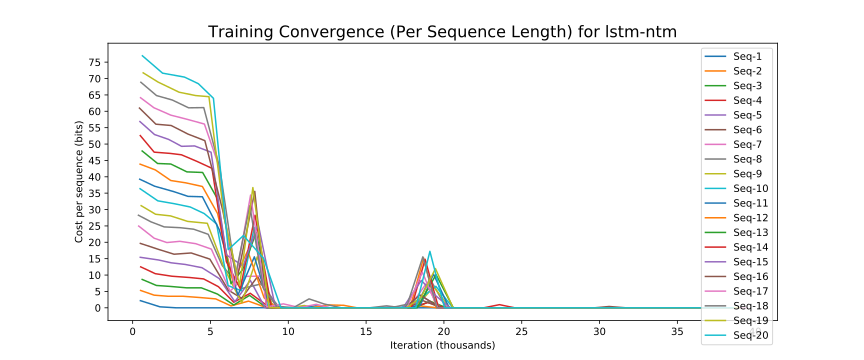
\includegraphics[width=100mm]{outputs/lstm-ntm_convergence-perlen}
\caption{Length-specific training curves of the LSTM-NTM.}
\label{Figure 5}
\end{figure}

\begin{figure}[h]
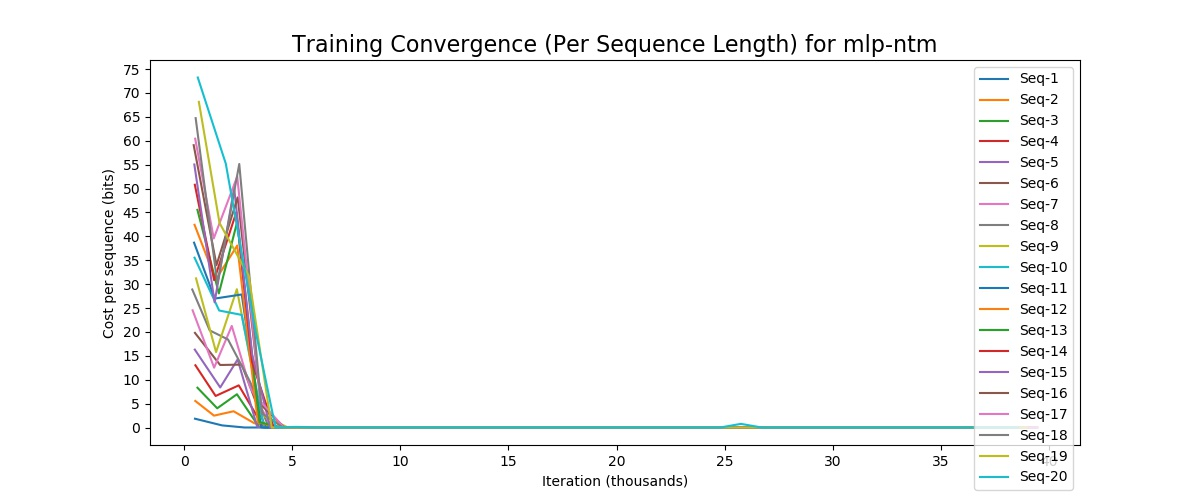
\includegraphics[width=100mm]{outputs/mlp-ntm_convergence-perlen}
\caption{Length-specific training curves of the MLP-NTM.}
\label{Figure 6}
\end{figure}

\begin{figure}[h]
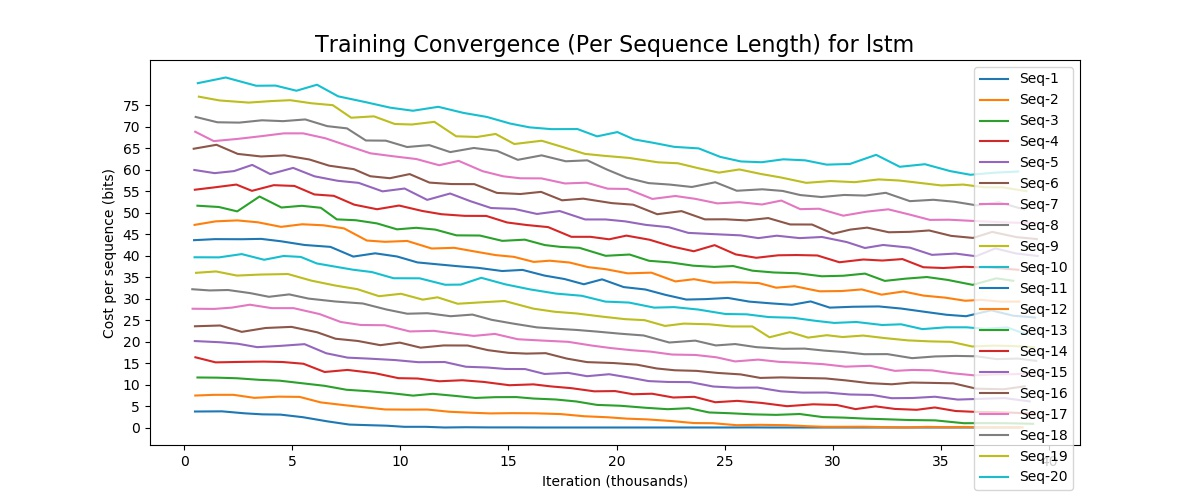
\includegraphics[width=100mm]{outputs/lstm_convergence-perlen}
\caption{Length-specific training curves of the LSTM baseline.}
\label{Figure 7}
\end{figure}

It can be seen that the MLP-NTM model converges fastest, followed by the
LSTM-NTM. The LSTM model improves over time, but does not converge nearly as
quickly as either NTM model, replicating the `qualitative' difference between
methods noted in the original paper. We speculate that the MLP-NTM converges
slightly faster because training an MLP generally takes less batches, and
is less sensitive to sample variance, than any recurrent model including
LSTM (of similar size). The baseline LSTM model likely did not converge
as quickly because of the slow leanring rate. The NTM variants likely
do not fare well with higher learning rates due to the powerful influence
of the memory matrix on the gradients, which the baseline LSTM model does
not have access to. However, it is also possible that the baseline LSTM
learning rate is approximately optimial, and the model is simply learning
the task as quickly as is possible for that architecture. \\

\subsection{Generalization to Longer Sequences} \\

For these three trained models, we tested their ability to correctly copy
binary sequences of length $T \in {10, 20, ..., 100}$, 20 times for each $T$.
We plot the mean and standard deviation across those 20 samples per T below
for the LSTM-NTM, MLP-NTM, and LSTM in figures 8-10: \\

\begin{figure}[h]
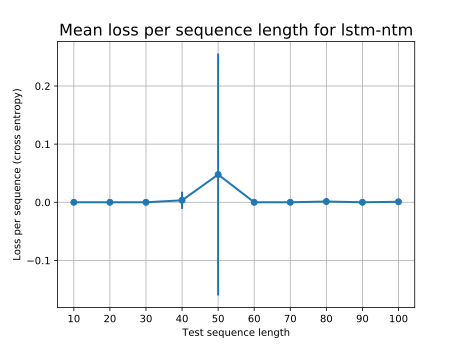
\includegraphics[width=100mm]{outputs/lstm-ntm_loss-eval}
\caption{Generalization to longer sequences for the LSTM-NTM.}
\label{Figure 8}
\end{figure}

\begin{figure}[h]
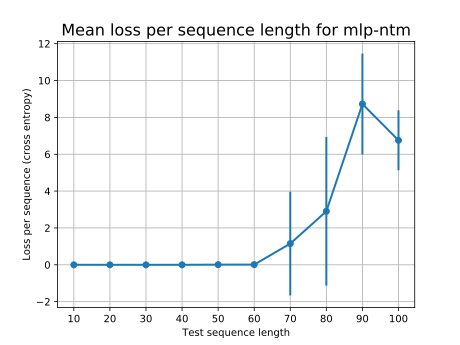
\includegraphics[width=100mm]{outputs/mlp-ntm_loss-eval}
\caption{Generalization to longer sequences for the MLP-NTM.}
\label{Figure 9}
\end{figure}

\begin{figure}[h]
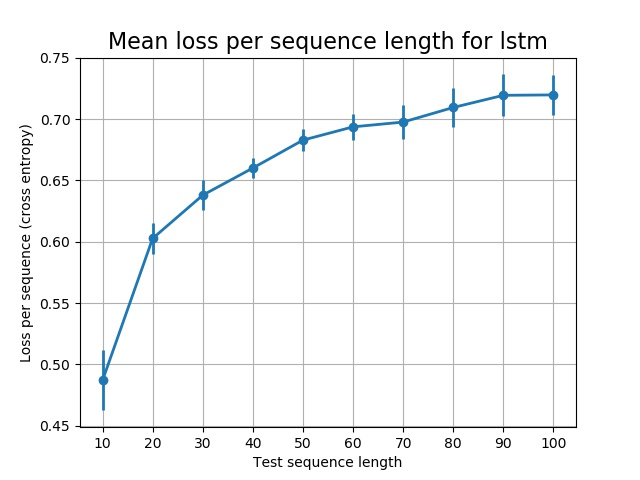
\includegraphics[width=100mm]{outputs/lstm_loss-eval}
\caption{Generalization to longer sequences for the LSTM baseline.}
\label{Figure 10}
\end{figure}

In this experiment, we expected both of the NTM models to be able to
generalize to all longer sequences, and the LSTM model to rapidly
degrade as sequence length gets longer. This is because we know
and expect recurrent models like the LSTM to have trouble composing
long sequences due to the vanishing/exploding gradients problem,
which leads to all recurrent models (to varying degrees) not being
able to learn very long-term dependencies. The NTM model gets around
this in a clever way: the memory module can store `chunks' of sequences
that the controller can then compose to generate a much larger sequence
than could typically be held in just the controller network.\\

This observation leads us to our results. Figure 8 clearly shows that
the MLP-NTM begins to falter as the sequence length reaches $T=50$,
while, the LSTM-NTM fares well at all sequence lengths, only showing
a small amount of weakness at $T=100$. The graph suggests good performance
of the LSTM-NTM for sequences much longer than $T=100$. We speculate
that this is because using a LSTM as the controller allows the NTM to
compose longer sequences of data held in the memory matrix than a MLP
controller given a fixed controller size (in this case, one hidden
layer of 100 nodes), since the LSTM is designed to learn sequences.
Said slightly differently, the optimial configuration for this task
uses an LSTM for the controller, which can learn how to sequence the
`chunked' memories held in the memory networks effectively, for
tasks that are sequential such as this one. We speculate that for
complex recognition tasks, an MLP or even convolutional architecture
in the controller would be useful, where the features stored in the
memory matrix represent sets of very high-order features that would
require an otherwise massive convolutional network to store effctively.\\

Unsuprisingly, the baseline LSTM model's performance quickly degrades
the sequence length increases, starting from $T=10$.\\


\subsection{Visualization of Read/Write Heads (Attention)} \\

We need a graph of the read/write heads. \\

\subsection{Understanding the Shift Operator} \\

We need the snippet of code using the shift operator, modification, etc. \\

\end{document}

